% Тип документа
\documentclass[a4paper,12pt]{extarticle}

% Шрифты, кодировки, символьные таблицы, переносы
\usepackage{cmap}
\usepackage[T2A]{fontenc}
\usepackage[utf8x]{inputenc}
\usepackage[russian]{babel}

% Это пакет -- хитрый пакет, он нужен но не нужен
\usepackage[mode=buildnew]{standalone}

\usepackage
	{
		% Дополнения Американского математического общества (AMS)
		amssymb,
		amsfonts,
		amsmath,
		amsthm,
		% misccorr,
		% 
		% Графики и рисунки
		wrapfig,
		graphicx,
		subcaption,
		float,
		tikz,
		tikz-3dplot,
		caption,
		csvsimple,
		color,
		booktabs,
		pgfplots,
		pgfplotstable,
		geometry,
		% 
		% Таблицы, списки
		makecell,
		multirow,
		indentfirst,
		%
		% Интегралы и прочие обозначения
		ulem,
		esint,
		esdiff,
		% 
		% Колонтитулы
		fancyhdr,
	}  


% Обводка текста в TikZ
\usepackage[outline]{contour}

% Увеличенный межстрочный интервал, французские пробелы
\linespread{1.3} 
\frenchspacing 

 
\usetikzlibrary
	{
		decorations.pathreplacing,
		decorations.pathmorphing,
		patterns,
		calc,
		scopes,
		arrows,
		fadings,
		through,
		shapes.misc,
		arrows.meta,
		3d,
		quotes,
		angles,
		babel
	}


\tikzset{
	force/.style=	{
		>=latex,
		draw=blue,
		fill=blue,
				 	}, 
	%				 	
	axis/.style=	{
		densely dashed,
		blue,
		line width=1pt,
		font=\small,
					},
	%
	th/.style=	{
		line width=1pt},
	%
	acceleration/.style={
		>=open triangle 60,
		draw=magenta,
		fill=magenta,
					},
	%
	inforce/.style=	{
		force,
		double equal sign distance=2pt,
					},
	%
	interface/.style={
		pattern = north east lines, 
		draw    = none, 
		pattern color=gray!60,
					},
	cross/.style=	{
		cross out, 
		draw=black, 
		minimum size=2*(#1-\pgflinewidth), 
		inner sep=0pt, outer sep=0pt,
					},
	%
	cargo/.style=	{
		rectangle, 
		fill=black!70, 
		inner sep=2.5mm,
					},
	%
	caption/.style= {
		midway,
		fill=white!20, 
		opacity=0.9
					},
	%
	}

\newenvironment{tikzpict}
    {
	    \begin{figure}[htbp]
		\centering
		\begin{tikzpicture}
    }
    { 
		\end{tikzpicture}
		% \caption{caption}
		% \label{fig:label}
		\end{figure}
    }


\newcommand{\vbLabel}[3]{\draw ($(#1,#2)+(0,5pt)$) -- ($(#1,#2)-(0,5pt)$) node[below]{#3}}
\newcommand{\vaLabel}[3]{\draw ($(#1,#2)+(0,5pt)$) node[above]{#3} -- ($(#1,#2)-(0,5pt)$) }

\newcommand{\hrLabel}[3]{\draw ($(#1,#2)+(5pt,0)$) -- ($(#1,#2)-(5pt,0)$) node[right, xshift=1em]{#3}}
\newcommand{\hlLabel}[3]{\draw ($(#1,#2)+(5pt,0)$) node[left, xshift=-1em]{#3} -- ($(#1,#2)-(5pt,0)$) }



\newcommand\zi{^{\,*}_i}
\newcommand\sumn{\sum_{i=1}^{N}}

\tikzset{
	coordsys/.style={scale=1.8,x={(1.1cm,-0cm)},y={(0.5cm,1cm)}, z={(0cm,0.8cm)}},
	coordsys/.style={scale=1.5,x={(0cm,0cm)},y={(1cm,0cm)}, z={(0cm,1cm)}}, 
	coordsys/.style={scale=1.5,x={(1cm,0cm)},y={(0cm,1cm)}, z={(0cm,0cm)}}, 
}

\usepgfplotslibrary{units}


% Draw line annotation
% Input:
%   #1 Line offset (optional)
%   #2 Line angle
%   #3 Line length
%   #5 Line label
% Example:
%   \lineann[1]{30}{2}{$L_1$}

\newcommand{\lineann}[4][0.5]{%
    \begin{scope}[rotate=#2, blue,inner sep=2pt, ]
        \draw[dashed, blue!40] (0,0) -- +(0,#1)
            node [coordinate, near end] (a) {};
        \draw[dashed, blue!40] (#3,0) -- +(0,#1)
            node [coordinate, near end] (b) {};
        \draw[|<->|] (a) -- node[fill=white, scale=0.8] {#4} (b);
    \end{scope}
}

\newcommand{\lineannn}[4][0.5]{%
    \begin{scope}[rotate=#2, blue,inner sep=2pt, ]
        \draw[dashed, blue!40] (0,0) -- +(0,#1)
            node [coordinate, near end] (a) {};
        \draw[dashed, blue!40] (#3,0) -- +(0,#1)
            node [coordinate, near end] (b) {};
        % \draw[color=white, color=blue] (a) -- node[fill=white, scale=0.8] {#4} (b);
        \draw[->|] (a)++(-0.3,0) -- (a);
        \draw[->|] (b)++(0.3,0) coordinate (xx) -- (b);
        \draw (xx) node[fill=white, scale=0.8, right] {#4};
    \end{scope}
}

% Круговая стрелка относительно центра (дуга из центра)
\tikzset{
  pics/carc/.style args={#1:#2:#3}{
    code={
      \draw[pic actions] (#1:#3) arc(#1:#2:#3);
    }
  },
  dash/.style={
  	dash pattern=on 5mm off 5mm
  }
}

% Среднее <#1>
\newcommand{\mean}[1]{\langle#1\rangle}

\pgfplotsset{
    % most recent feature set of pgfplots
    compat=newest,
}

% const прямым шрифтом
\newcommand\ct[1]{\text{\rmfamily\upshape #1}}
\newcommand*{\const}{\ct{const}}


\usepackage[europeanresistors,americaninductors]{circuitikz}

% Style to select only points from #1 to #2 (inclusive)
\pgfplotsset{select/.style 2 args={
    x filter/.code={
        \ifnum\coordindex<#1\def\pgfmathresult{}\fi
        \ifnum\coordindex>#2\def\pgfmathresult{}\fi
    }
}}


\usepackage{array}



%%%%%%%%%%%%%%%%%%%%%%%%%%%%%%%%%%%%%%%%%%%%%%%%%
\makeatletter
\newif\if@gather@prefix 
\preto\place@tag@gather{% 
  \if@gather@prefix\iftagsleft@ 
    \kern-\gdisplaywidth@ 
    \rlap{\gather@prefix}% 
    \kern\gdisplaywidth@ 
  \fi\fi 
} 
\appto\place@tag@gather{% 
  \if@gather@prefix\iftagsleft@\else 
    \kern-\displaywidth 
    \rlap{\gather@prefix}% 
    \kern\displaywidth 
  \fi\fi 
  \global\@gather@prefixfalse 
} 
\preto\place@tag{% 
  \if@gather@prefix\iftagsleft@ 
    \kern-\gdisplaywidth@ 
    \rlap{\gather@prefix}% 
    \kern\displaywidth@ 
  \fi\fi 
} 
\appto\place@tag{% 
  \if@gather@prefix\iftagsleft@\else 
    \kern-\displaywidth 
    \rlap{\gather@prefix}% 
    \kern\displaywidth 
  \fi\fi 
  \global\@gather@prefixfalse 
} 
\newcommand*{\beforetext}[1]{% 
  \ifmeasuring@\else
  \gdef\gather@prefix{#1}% 
  \global\@gather@prefixtrue 
  \fi
} 
\makeatother
%%%%%%%%%%%%%%%%%%%%%%%%%%%%%%%%%%%%%%%%%%%%%%%%%

\geometry		
	{
		left			=	2cm,
		right 			=	2cm,
		top 			=	3cm,
		bottom 			=	3cm,
		bindingoffset	=	0cm
	}

%%%%%%%%%%%%%%%%%%%%%%%%%%%%%%%%%%%%%%%%%%%%%%%%%%%%%%%%%%%%%%%%%%%%%%%%%%%%%%%



	%применим колонтитул к стилю страницы
\pagestyle{fancy} 
	%очистим "шапку" страницы
\fancyhead{} 
	%слева сверху на четных и справа на нечетных
\fancyhead[R]{\labauthors} 
	%справа сверху на четных и слева на нечетных
\fancyhead[L]{Отчёт по лабораторной работе №\labnumber} 
	%очистим "подвал" страницы
\fancyfoot{} 
	% номер страницы в нижнем колинтуле в центре
\fancyfoot[C]{\thepage} 

%%%%%%%%%%%%%%%%%%%%%%%%%%%%%%%%%%%%%%%%%%%%%%%%%%%%%%%%%%%%%%%%%%%%%%%%%%%%%%%

\renewcommand{\contentsname}{Оглавление}

\usepackage{tocloft}
% \renewcommand{\cftpartleader}{\cftdotfill{\cftdotsep}} % for parts
% \renewcommand{\cftsectiondotsep}{\cftdotsep}% Chapters should use dots in ToC
\renewcommand{\cftsecleader}{\cftdotfill{\cftdotsep}}
%\renewcommand{\cftsecleader}{\cftdotfill{\cftdotsep}} % for sections, if you really want! (It is default in report and book class (So you may not need it).
% ---------
% \newcommand{\cftchapaftersnum}{.}%
% \usepackage{titlesec}
% \titlelabel{\thetitle.\quad}
\usepackage{secdot}
\sectiondot{subsection}
\usepackage{colortbl}
\begin{document}

\def\labauthors{Понур К.А., Сарафанов Ф.Г., Сидоров Д.А.}
\def\labgroup{420}
\def\labnumber{204}
\def\labtheme{Эффект Холла}
\renewcommand{\vec}{\mathbf}
\begin{titlepage}

\begin{center}

{\small\textsc{Нижегородский государственный университет имени Н.\,И. Лобачевского}}
\vskip 1pt \hrule \vskip 3pt
{\small\textsc{Радиофизический факультет}}

\vfill

{\Large Отчет по лабораторной работе №\labnumber\vskip 12pt\bfseries \labtheme}
	
\end{center}

\vfill
	
\begin{flushright}
	{Выполнили студенты \labgroup\ группы\\ \labauthors}%\vskip 12pt Принял:\\ Менсов С.\,Н.}
\end{flushright}
	
\vfill
	
\begin{center}
	Нижний Новгород, \the\year
\end{center}

\end{titlepage}



\tableofcontents
\newpage

\section*{Введение}
\addcontentsline{toc}{section}{Введение}
\label{sec:input}

В данной работе исследуется эффект Холла.

Эффект Холла представляет собой в появление поперечной э.д.с. при прохождении 
электрического тока через проводник, помещенный в магнитное поле, перпендикулярное к направлению тока. 

Измерение холловской разности потенциалов обычно позволяет определить концентрацию и знак основных носителей заряда в веществе.

Целью данной работы является изучение возникновения эффекта Холла в слабом магнитном поле, определение коэффициента Холла, холловской подвижности, определение концентрации основных носителей в образце.

\section{Анализ теории}
\subsection[Описание эффекта Холла]{Описание эффекта Холла без учёта механизма рассеяния носителей заряда}
\subsubsection{Разделение зарядов}
Рассмотрим образец, через который протекает ток $\vec{j}$.
\begin{figure}[H]
	\centering
	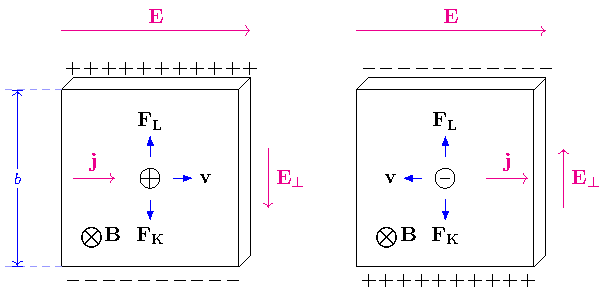
\includegraphics[width=0.85\textwidth]{img/effect}
	\caption{Механизм разделения зарядов при проявлении эффекта Холла}
	\label{fig:figure1}
\end{figure}

Электрическое поле $\vec{Е}$ создает в полупроводнике электрический ток плотностью 
\begin{equation}
	\vec{j}=\sigma\vec{E},
\end{equation}
где $\sigma=\frac{1}{\rho}$ -- удельная электрическая проводимость, $\rho$ -- удельное сопротивление проводника. 

Со стороны магнитного поля В на движущиеся заряды действует магнитная составляющая силы Лоренца 
\begin{equation}
	\label{eq:fl}
	\vec{F}_L=q[\vec{v}\times\vec{B}]
\end{equation}
Здесь $\vec{v}$ - дрейфовая скорость носителей заряда.

Под действием этой силы происходит разделение зарядов на противоположных боковых (параллельных току и магнитному полю) гранях образца.

При разделении зарядов грани заряжаются, и возникает поперечное поле $\vec{E}_\perp$ -- поле Холла. На заряд начинает действовать сила Кулона
\begin{equation}
	\vec{F}_K=q\vec{E}_\perp
\end{equation}

\subsubsection{Равновесное состояние}

Поле Холла препятствует движению зарядов, вызванным действием магнитного поля, и на некотором этапе разделения зарядов наступает равновесие сил $\vec{F}_K$ и $\vec{F}_L$:
\begin{equation}
	\label{eq:eq}
	q\vec{E}_\perp+\vec{F}_L=0
\end{equation}

Отсюда
\begin{equation}
	\label{eq:ep}
	\vec{E}_\perp=-[\vec{v}\times\vec{B}]
\end{equation}

Обозначим плотность тока:
\begin{equation}
j=\frac{I}{S}
\end{equation}
Распишем ток:
\begin{equation}
I=\frac{dQ}{dt}=\frac{qnvS\,dt}{dt}=qnvS,
\end{equation}
где $n$ - концентрация заряда по объему.

Отсюда
\begin{equation}
v=\frac{I}{qnS}=\frac{j}{qn}=\frac{\sigma E}{qn}
\end{equation}
То есть
\begin{equation}
	\label{eq:mue}
	v\sim E
	\quad\Rightarrow\quad
	\vec{v}=\mu \vec E, \quad \mu=\frac{\sigma}{qn}
\end{equation}

Из (\ref{eq:ep}), (\ref{eq:mue}) следует
\begin{equation}
	\label{eq10}
	\vec{E}_\perp=-\mu[\vec{E}\times\vec{B}]
\end{equation}
Или с учетом $\vec{j}=\sigma\vec{E}$
\begin{equation}
	\vec{E}_\perp=-R[\vec{j}\times\vec{B}]
\end{equation}

Где $R$ -- коэффициент Холла.

\subsubsection{Коэффициент Холла}
В нашем выводе
\begin{equation}
	R\sigma=\mu
	\quad \Rightarrow\quad
	R=\frac{1}{qn}
\end{equation}

При более строгом выводе, учитывающем механизм рассеяния свободных носителей заряда, можно получить 
\begin{equation}
	R=\frac{\gamma}{qn}
\end{equation}

Где $\gamma$ -- холл-фактор, безразмерный коэффициент, зависящий от величины магнитного поля и механизма рассеяния свободных носителей заряда при их взаимодействии с ионами примесей и кристаллической решеткой. 

Для используемого в данной лабораторной работе чистого слабо легированного германия при комнатной температуре в слабом магнитном поле $\gamma\approx 1.18$.

\subsubsection{Холловская подвижность}

Произведение $R\sigma$ имеет размерность подвижности и называется холловской подвижностью:
\begin{equation}
	\mu_H=R\sigma
\end{equation}

\subsubsection{Угол Холла}

Действие магнитного поля $\vec{B}$ приводит к тому, что суммарное электрическое поле 
\begin{equation}
	\vec{E}_\Sigma=\vec{E}+\vec{E}_\perp
\end{equation}
оказывается повернутым на некоторый угол $\vartheta$ (угол Холла) относительно вектора плотности тока. Из полученных ранее выражений можно показать, что
\begin{equation}
	\tan\vartheta=-\mu_H B
\end{equation}
При слабом магнитном поле 
\begin{equation}
	-\mu_H B \ll 1
\end{equation}
 угол Холла приближенно можно вычислить по формуле 
\begin{equation}
	\vartheta=-\mu_H B
\end{equation}

\subsubsection{Холловская разность потенциалов}

Эквипотенциальные поверхности в средней части ограниченного вытянутого образца поворачиваются при включении магнитного поля В на угол $\vartheta$ относительно их первоначального положения.

Из-за этого в точках, изначально лежащих на эквипотенциали, появляется разность потенциалов $U_H$, называемая холловской разностью потенциалов.

Для образца прямоугольной формы в приближении однородного поля Холла эта разность потенциалов будет равна 
\begin{equation}
	U_H=bE_\perp
\end{equation}

Для прямоугольного образца
\begin{equation}
	j=\frac{I}{S}=\frac{I}{bc}
\end{equation}
Из (\ref{eq:mue}), (\ref{eq10}) следует
\begin{equation}
	{E}_\perp=\frac{j}{qn}B
\end{equation}
Откуда
\begin{equation}
	\frac{U_H}{b}=\frac{I}{qn\cdot bc}B
\end{equation}
И окончательно
\begin{equation}
	U_H=\frac{R}{c}IB
\end{equation}

\subsection{Побочные факторы}
\subsubsection{Нехолловская составляющая измеряемой разности потенциалов}

При изготовлении образца не удается разместить оба холловских контакта таким образом, чтобы они в отсутствие магнитного поля лежали на одной эквипотенциальной поверхности. 

В реальном образце между плоскостями расположения контактов всегда есть небольшое смещение $\Delta x$. 

При $\vec{B}=0$ и $I\ne0$ между этими плоскостями устанавливается разность потенциалов, равная 
\begin{equation}
	U_{34}=R_{34}I,
	\text{  где  }
	R_{34}=\rho\frac{\Delta x}{bc}
\end{equation}

Другие побочные факторы дают вклад в разность потенциалов между контактами 3 и 4 существенно меньший холловской разности потенциалов. 

Таким образом, в рамках нашей модели справедливо выражение
\begin{equation}
	U_H=U_{34}|_{B\ne 0}-U_{34}|_{B= 0}=\frac{RIB}{c}
\end{equation}

Отсюда видно, что коэффициент Холла $К$ может быть определен по тангенсу угла наклона линейных участков экспериментально снятых зависимостей $U_{34}(B)|_{I=\const}$ и $U_H(I)|_{B=\const}$.

\section{Экспериментальные данные}
\subsection{Вольт-амперная характеристика участка $R_{56}$}

Была снята зависимость разности потенциалов контактов 5 и 6 от
величины тока в отсутствие магнитного поля В. Измерения проведены для
двух направлений тока при изменении его величины от 0 до 10 мА. 

\begin{figure}[H]
	\centering
	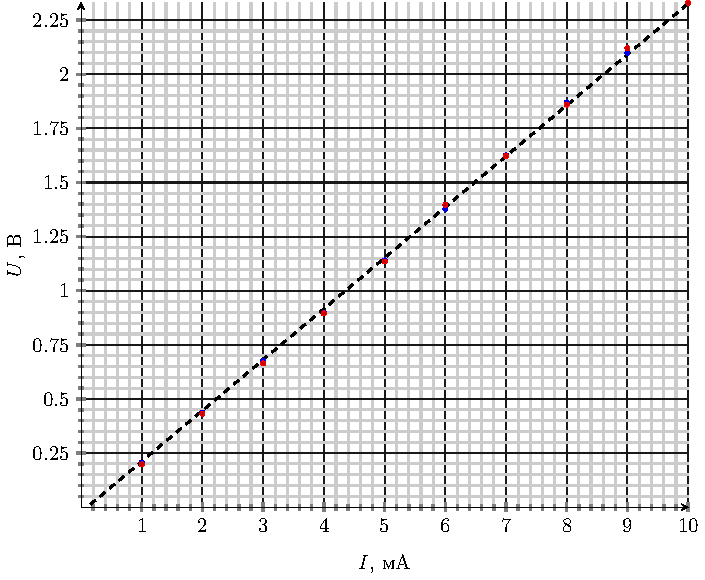
\includegraphics[width=\textwidth]{img/vax}
	\caption{ВАХ элемента}
	\label{fig:vax}
\end{figure}

Из графика определено сопротивление участка $R_{56}$:
\begin{equation}
	R_{56}=(237\pm 2) \text{ Ом}
\end{equation}

Используя данные о поперечных размерах образца, расстоянии между контактами и значении $R_{56}$, можно вычислить удельную электрическую проводимость полупроводника в единицах $\text{Ом}^{-1}\text{см}^{-1}$.
\begin{equation}
	\sigma=\frac{1}{\rho} =\frac{l_{56}}{R_{56} \cdot S}=\frac{d}{R_{56}\cdot bc}=\frac{0.96}{237\cdot 0.48\cdot 0.102}=0.0827 \text{ Ом}^{-1}\text{см}^{-1}
\end{equation}

\subsection{Определение знака холловской разности потенциалов}

При установленном токе в образце $J^{+}=5$ мА измерена разность потенциалов между
контактами 3-4 при выключенном магнитном поле и при поле $B^{+}=2000$ Гс:
\begin{equation}
	\Delta\varphi|_{B=0}=0.0297 \text{ В}
\end{equation}
\begin{equation}
	\Delta\varphi|_{B=2000+ \text{Гс}}=0.0063 \text{ В}
\end{equation}
По результатам измерений определен знак и величина холловской разности потенциалов:
\begin{equation}
	U_H=\Delta\varphi|_{B=2000+ \text{Гс}}-\Delta\varphi|_{B=0}=0.0063-0.0297=-0.0234 \text{ В}
\end{equation}
а также знак основных носителей заряда в образце - положительный, значит носителями заряда являются дырки.

\subsection{Определение коэффициента Холла}
\subsubsection{Определение зависимости $U^B_{34}(B)|_{J=const}$}
Установив ток в образце ${J=2\,\text{мА}}$, Сняли зависимость разности потенциалов $U^B_{34}$ от величины поля $B$. Измерения проведены  при изменении тока $i$ в обмотках электромагнита 0 до 1 А с шагом 0.1 А. Эксперимент повторили для ${J=5\,\text{мА}}$, ${J=8\,\text{мА}}$.

%!TEX root=record.tex
\begin{table}[H]
	    \caption{Зависимость $U_{34}(B)$}
	    \label{tab:diod}
	    \pgfkeys{/pgf/number format/.cd,
		fixed,  1000 sep={\,}}
\newlength\Colsep
\setlength\Colsep{10pt}
% \xdef\Table{data/i.tsv}
\pgfplotstableset{
	% multicolumn names, % allows to have multicolumn names
	% header=has colnames,
	dec sep align,
	col sep=tab, % the seperator in our .csv file
	fixed zerofill, 
	precision=4,
	columns/i/.style={
		column name={$i$, А},
		precision=1,		
	},	
	columns/ubp2/.style={
		column name={$U|_{J=+2\,\text{мА}}$, В},
		% column type/.add={|}{},
	},
	columns/ubm2/.style={
		column name={$U|_{J=-2\,\text{мА}}$, В},
		% column type/.add={}{|}
	},
	columns/ubp5/.style={
		column name={$U|_{J=+5\,\text{мА}}$, В},
	},	
	columns/ubm5/.style={
		column name={$U|_{J=-5\,\text{мА}}$, В},
		% column type/.add={}{|}
	},		
	columns/ubp8/.style={
		column name={$U|_{J=+8\,\text{мА}}$, В},
	},
	columns/ubm8/.style={
		column name={$U|_{J=-8\,\text{мА}}$, В},
	},
	empty cells with={\textbf{--}},
	every head row/.style={
	before row={\toprule},
	after row={
		\midrule}
		},
	every last row/.style={after row=\bottomrule},
	every row/.style={after row=\midrule}, 
	columns={i,ubp2,ubm2,ubp5,ubm5,ubp8,ubm8	},		
	% dec zerofill
	% fixed,fixed zerofill,
	% precision=3
	every even column/.style={
		% column type/.add={>{\columncolor[gray]{.8}}}{}
	},
	every even row/.style={
		before row={\rowcolor[gray]{0.95}}
	},	
	}

\centering
	\pgfplotstabletypeset[]{data/i.tsv}

\end{table}

\begin{figure}[H]
	\centering
	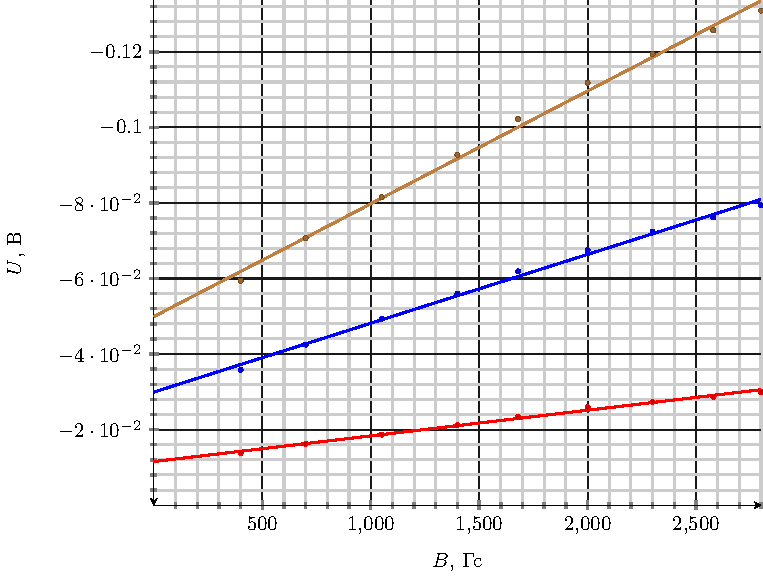
\includegraphics[width=0.89\textwidth]{img/n10m}
	% \caption{}
	\label{fig:uhp}
\end{figure}

\begin{figure}[H]
	\centering
	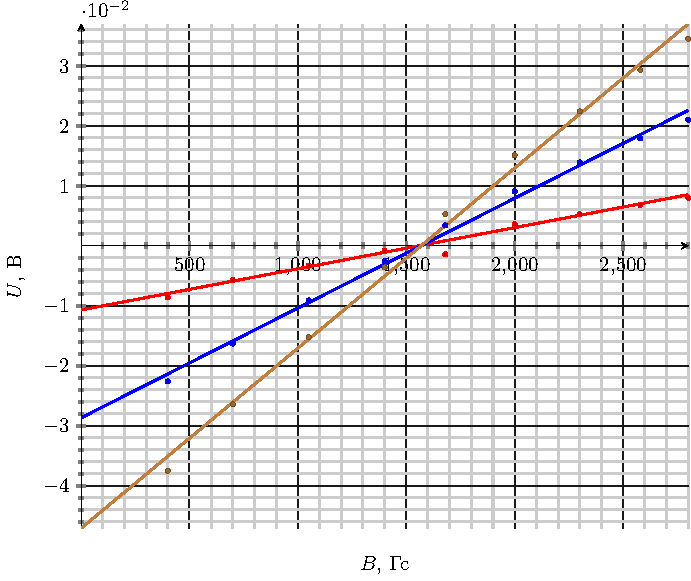
\includegraphics[width=0.79\textwidth]{img/n10p}
	% \caption{}
	\label{fig:uhm}
\end{figure}

Для трех токов нашли угловой коэффициент:
\begin{equation}
	\frac{U_H}{B}\bigg|_{J=2\text{ мА}}=0.68\cdot10^{-2}\ \frac{\text{мВ}}{\text{Гс}},\quad
	\frac{U_H}{B}\bigg|_{J=5\text{ мА}}=1.83\cdot10^{-2}\ \frac{\text{мВ}}{\text{Гс}},\quad
	\frac{U_H}{B}\bigg|_{J=8\text{ мА}}=3\cdot10^{-2}\ \frac{\text{мВ}}{\text{Гс}}
\end{equation}

Отсюда
\begin{equation}
	R=\frac{U_H}{B}\frac{c}{J}=0.68\cdot10^{-2}\ \frac{\text{мВ}}{\text{Гс}}\cdot \frac{0.102\text{ см}}{8 \text{ мА}}\cdot 10^8=
	0.68\cdot10^{-2}\cdot \frac{0.102}{2}\cdot 10^8=34680\ \frac{\text{см}^3}{\text{Кл}}
\end{equation}
Аналогично
\begin{equation}
	R=1.83\cdot10^{-2}\cdot \frac{0.102}{5}\cdot 10^8=37332\ \frac{\text{см}^3}{\text{Кл}}
\end{equation}
\begin{equation}
	R=3\cdot10^{-2}\cdot \frac{0.102}{8}\cdot 10^8=38250\ \frac{\text{см}^3}{\text{Кл}}
\end{equation}

\subsubsection{Определение зависимости $U_{H}(J)|_{B=const}$}

Сняли зависимость $U_{H}(J)|_{B=const}$. Измерения провели при выключенном
магнитном поле, а затем при четырех различных значениях $B^{+}$.
Нашли угловой коэффициент:
\begin{gather}
	\frac{U_H}{J}\bigg|_{B=650\text{ Гс}}=2.315\ \frac{\text{мВ}}{\text{мА}},\quad
	\frac{U_H}{J}\bigg|_{B=1500\text{ Гс}}=5.696\ \frac{\text{мВ}}{\text{мА}},\\
	\frac{U_H}{J}\bigg|_{B=2000\text{ Гс}}=7.622\ \frac{\text{мВ}}{\text{мА}},\quad
	\frac{U_H}{J}\bigg|_{B=2400\text{ Гс}}=8.886\ \frac{\text{мВ}}{\text{мА}}
\end{gather}
\begin{figure}[H]
	\centering
	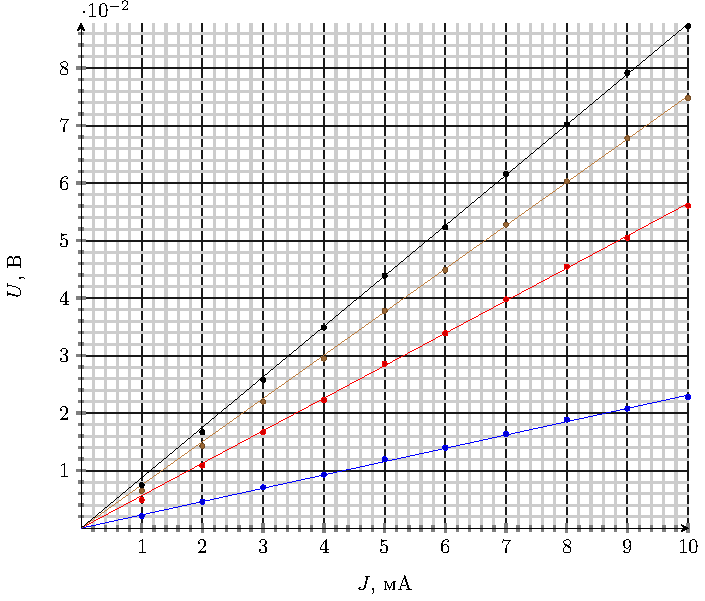
\includegraphics[width=0.79\textwidth]{img/UHp}
	% \caption{}
	\label{fig:uhp}
\end{figure}
\begin{figure}[H]
	\centering
	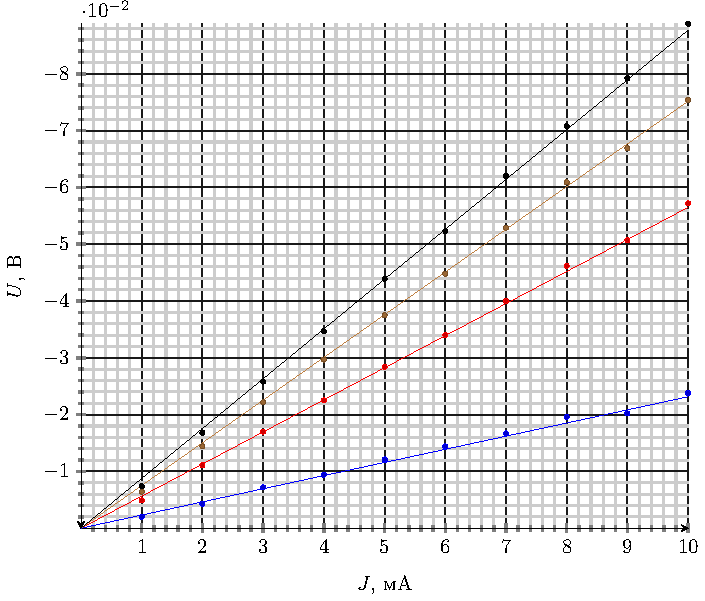
\includegraphics[width=0.79\textwidth]{img/UHm}
	% \caption{}
	\label{fig:uhm}
\end{figure}
Отсюда
\begin{equation}
	R=\frac{U_H}{J}\frac{c}{B}=2.315\ \frac{\text{мВ}}{\text{мА}}\cdot \frac{0.102\text{ см}}{650 \text{ Гс}}\cdot 10^8=
	2.315\cdot \frac{0.102}{650}\cdot 10^8=36327\ \frac{\text{см}^3}{\text{Кл}}
\end{equation}
Аналогично
\begin{equation}
	R=5.696\cdot \frac{0.102}{1500}\cdot 10^8=38732\ \frac{\text{см}^3}{\text{Кл}}
\end{equation}
\begin{equation}
	R=7.622\cdot \frac{0.102}{2000}\cdot 10^8=38872\ \frac{\text{см}^3}{\text{Кл}}
\end{equation}
\begin{equation}
	R=8.886\cdot \frac{0.102}{2400}\cdot 10^8=37765\ \frac{\text{см}^3}{\text{Кл}}
\end{equation}

Среднее значение $R$ по всем экспериментам
\begin{equation}
	R\equiv\mean{R}=37400\ \frac{\text{см}^3}{\text{Кл}}
\end{equation}

\subsubsection{Определение сопротивления участка $R_{34}$}
\begin{figure}[H]
	\centering
	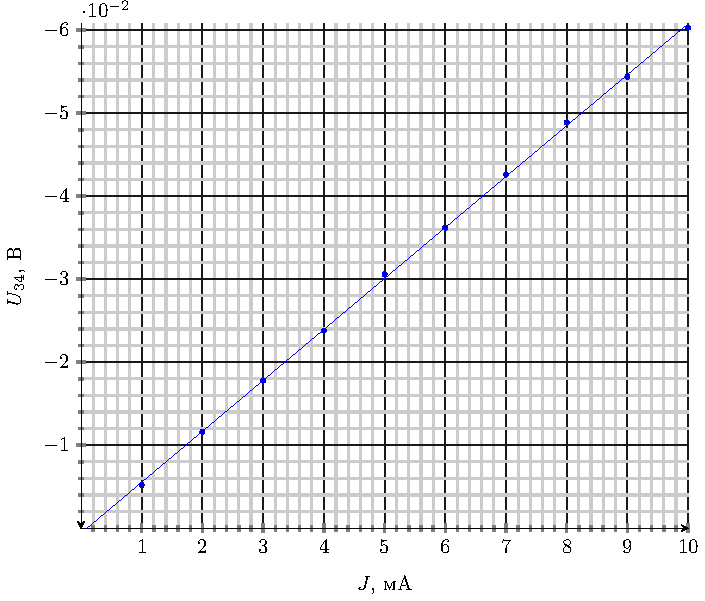
\includegraphics[width=0.79\textwidth]{img/U34}
	% \caption{}
	\label{fig:uhm}
\end{figure}
Из графика $U_{34}(J)|_{B=0}$ нашли сопротивление $R_{34}$ как угловой коэффициент:
\begin{equation}
	R_{34}=6.137\ \frac{\text{мВ}}{\text{мА}}=6.137 \text{ Ом}
\end{equation}
Тогда можем найти смещение:
\begin{equation}
	\Delta x=bc\cdot R_{34}\cdot \sigma=0.48\cdot0.102\cdot6.137\cdot 0.0827=0.025 \text{ cм}
\end{equation}

\subsection{Определение холловской подвижности и угла Холла}

Найдем холловскую подвижность:
\begin{equation}
	\mu_H=R\sigma=37400\cdot0.0827=3092\ \frac{\text{см}^2}{\text{Кл}\cdot \text{Ом}}
\end{equation}
\begin{equation}
	\mu_H=0.3\ \frac{\text{м}^2}{\text{Кл}\cdot \text{Ом}}
\end{equation}

Проверим условие слабого поля. В нашем случае поле порядка 3000 Гс (0.3 Тл):
\begin{equation}
	\mu_H\cdot B=0.3\cdot0.3=0.09 \ll 1
\end{equation}

Для поля 2000 Гс можем найти угол Холла:
\begin{equation}
	\vartheta\approx-\mu_H\cdot B=-0.3\cdot0.2=-0.06
\end{equation}

\subsection{Определение концентрации носителей}

Оценим концентрацию носителей по формуле
\begin{equation}
	n=\frac{\gamma}{Rq}
\end{equation}
Здесь $\gamma$ -- холл-фактор, учитывающий механизм рассеяния свободных носителей заряда, для используемого образца $\gamma=1.18$:
\begin{equation}
	n=\frac{1.18\cdot10^{19}}{37400\cdot1.6}=1.97\cdot10^{14}
\end{equation}

\newpage
\section{Заключение}

В ходе данной работы была снята зависимость разности потенциалов контактов 5 и 6 от
величины тока в отсутствие магнитного поля В. Определено сопротивление участка $R_{56}$:
\begin{equation}
	R_{56}=(237\pm 2) \text{ Ом}
\end{equation}

Вычислена удельная электрическая проводимость полупроводника
\begin{equation}
	\sigma=0.0827 \text{ Ом}^{-1}\text{см}^{-1}
\end{equation}

Определен знак и величина холловской разности потенциалов, а также знак основных носителей заряда в образце: положительный -- значит, носителями заряда являются дырки.

Сняли зависимость разности потенциалов $U^B_{34}$ от величины поля $B$.
Так же сняли зависимость $U_{H}(J)|_{B=const}$.

Анализом графиков получили среднее значение коэффициента Холла $R$
\begin{equation}
	R\equiv\mean{R}=37400\ \frac{\text{см}^3}{\text{Кл}}
\end{equation}

Из графика $U_{34}(J)|_{B=0}$ нашли сопротивление $R_{34}$ как угловой коэффициент:
\begin{equation}
	R_{34}=6.137 \text{ Ом}
\end{equation}

Нашли смещение контактов:
\begin{equation}
	\Delta x=0.025 \text{ cм}
\end{equation}

Определили холловскую подвижность
\begin{equation}
	\mu_H=0.3\ \frac{\text{м}^2}{\text{Кл}\cdot \text{Ом}}
\end{equation}

Для поля 2000 Гс нашли угол Холла:
\begin{equation}
	\vartheta=-0.06
\end{equation}

Оценили концентрацию свободных носителей
\begin{equation}
	n=1.97\cdot10^{14}
\end{equation}

% В ходе данной работы был определен коэффициент Холла $\frac{\text{см^3}}{\text{Кл}}$. Был найден угол Холла при $B=2000\text{Гс}\phi=0.17$ и подвижность $ \mu_H=0.3092 $ 
% Также мы выяснили, что полупроводник обладает дырочной проводимостью и нашли концентрацию носителей заряда в образце.

\end{document}